\documentclass[10pt,xcolor=pdflatex,hyperref={unicode}]{beamer}
\usepackage{newcent}
\usepackage[utf8x]{inputenc}
\usepackage[T1]{fontenc}
\usepackage{hyperref}
\usepackage{fancyvrb}
\usepackage{tikz}
\usepackage{tikz-cd}
\usepackage{listings}
\usepackage{graphicx}
\usepackage{textcomp}
\usepackage{minted}

\usetheme{FIT}

\title[$\Lambda\Pi$ JIT]{Just-in-Time Compilation of the Dependently-Typed Lambda Calculus}
\author[]{Jakub Zárybnicky <xzaryb00@stud.fit.vutbr.cz>}
\institute[]{Brno University of Technology, Faculty of Information Technology\\
Bo\v{z}et\v{e}chova 1/2. 612 66 Brno - Kr\'alovo Pole\\
login@fit.vutbr.cz}
\date{\today}

\begin{document}
\frame[plain]{\titlepage}

\begin{frame}\frametitle{Motivation}
  \begin{itemize}
  \item Writing programming languages
  \end{itemize}
  \medskip
  \begin{tabular}{l l}
    Compiler & Interpreter \\
    \hline
    \textbf{Fast}  & Slow  \\
    Hard(er)-to-create  & \textbf{Easy-to-create}  \\
  \end{tabular}
  \pause
  \medskip
  \begin{itemize}
  \item Third way - JIT compilation, write an interpreter, maybe add runtime optimizations
  \end{itemize}
\end{frame}

\begin{frame}\frametitle{JIT compilation}
\begin{figure}
\begin{tikzcd}[ampersand replacement=\&]
{} \& Program
 \arrow[ld, "Compiler" description, bend right]
 \arrow[dd, "Interpreter" description, bend right=67]
 \arrow[rd, "Partial\ Evaluation" description, bend left]
 \arrow[dd, "JIT" description, bend left=67] \& {} \\
Executable \arrow[rd, "Run" description, bend right] \& {} \& Native\ Image \arrow[ld, "Run", bend left]
 \\ {} \& Result \& {}
\end{tikzcd}
\caption{Methods of program execution}
\label{fig:futamora}
\end{figure}
\end{frame}

\begin{frame}\frametitle{GraalVM}
\begin{figure}[!htpb]
\centering
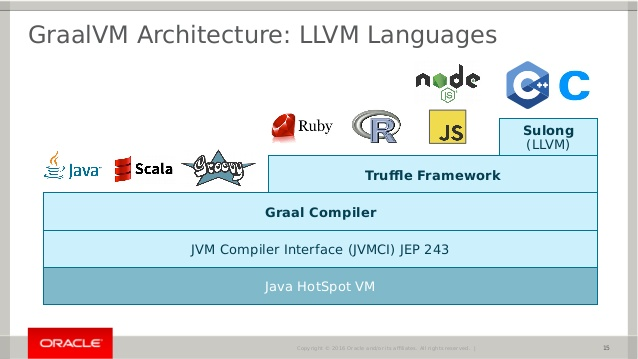
\includegraphics[width=.9\linewidth]{./img/graalvm.jpg}
\caption{GraalVM and Truffle (source: oracle.com)}
\end{figure}
\end{frame}

\begin{frame}\frametitle{JIT compilation}
\begin{figure}
\centering
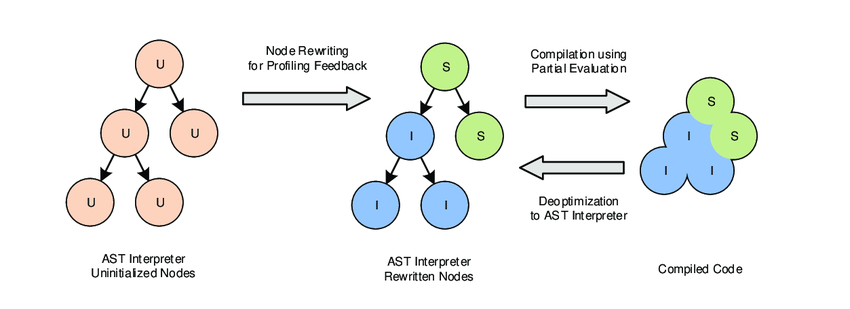
\includegraphics[width=.9\linewidth]{./img/node-rewrite.png}
\caption{Node rewriting (src: Truffle DSL, 10.13140/RG.2.2.23639.52646)}
\end{figure}
\end{frame}

\begin{frame}\frametitle{$\Lambda\Pi-calculus$}
  \begin{figure}
    \begin{equation}
\begin{array}{ccll}
e & ::= & x           & \text{variable} \\
  & |   & e_1~e_2      & \text{application} \\
  & |   & \lambda x. e & \text{abstraction} \\
  & |   & x:\tau      & \text{annotation} \\
  & |   & *           & \text{the type of types} \\
  & |   & \forall x:\rho.\rho' & \text{dependent function space}
\end{array}
\end{equation}
  \caption{Dependently typed lambda calculus}
\end{figure}
\end{frame}

\begin{frame}[fragile]\frametitle{$\Lambda\Pi-calculus$}
\begin{verbatim}
let const = (\ a b x y -> x)
   :: forall (a :: *) (b :: *) . a -> b -> a
\end{verbatim}
\end{frame}

\begin{frame}\frametitle{Assignment}
\begin{enumerate}
\item Investigate dependent types, simply-typed and dependently-typed lambda
calculus, and their evaluation models (push/enter, eval/apply).
\item Get familiar with the Graal virtual machine and the Truffle language
implementation framework.
\item Create a parser, and an interpreter for a selected language based on
dependently-typed lambda calculus.
\end{enumerate}
\end{frame}

\begin{frame}\frametitle{Implementations}
  \begin{itemize}
    \item Interpreter (plain Kotlin), 100\% done
    \item JIT compiler (Kotlin + Truffle), 10\% done
    \item LLVM compiler (Kotlin + LLVM bindings), 5\% done
  \end{itemize}
\end{frame}

\bluepage{Thank You For Your Attention !}

\end{document}

%%% Local Variables:
%%% mode: latex
%%% TeX-master: t
%%% End:
